\documentclass[11pt,a4paper]{article}

% These are extra packages that you might need for writing the equations:
\usepackage{amsmath}
\usepackage{amsfonts}
\usepackage{amssymb}
\usepackage{booktabs}
\usepackage{hyperref}
\usepackage{listings}
\usepackage{xcolor}
\lstset {language=C++,
		 basicstyle=\ttfamily,
         keywordstyle=\color{blue}\ttfamily,
         stringstyle=\color{red}\ttfamily,
         commentstyle=\color{purple}\ttfamily,
         morecomment=[l][\color{magenta}]{\#},
       	 basicstyle=\tiny}

% You need the following package in order to include figures in your report:
\usepackage{graphicx}

% With this package you can set the size of the margins manually:
\usepackage[left=2cm,right=2cm,top=2cm,bottom=2cm]{geometry}


\begin{document}

% Enter the exercise number, your name and date here:
\noindent\parbox{\linewidth}{
 \parbox{.25\linewidth}{ \large ICP, Exercise 05 }\hfill
 \parbox{.5\linewidth}{\begin{center} \large Beat Hubmann \end{center}}\hfill
 \parbox{.2\linewidth}{\begin{flushright} \large Oct 27, 2018 \end{flushright}}
}
\noindent\rule{\linewidth}{2pt}


\section{Introduction}

A Monte Carlo method to approximate the high-dimensional conditioned integration to calculate the average distance
between the centers of hard spheres in a box was implemented and examined for convergence.

\section{Algorithm Description}
To calculate the average sphere center distance as in equation~\ref{eqn:1}, the Monte Carlo approximation as in equation~\ref{eqn:2}
is calculated. The algorithm was implemented as in the written task description except for one change: Based on instructor suggestion,
a new configuration is generated in one go: $ n \cdot \text{\# dim} $ random numbers are generated in a contiguous batch and the resulting
configuration only then gets checked for validity. If an overlap between spheres is found, the complete configuration is thrown away and
 a new one is generated with a different random number generator seed. This is repeated until a valid configuration is found or 
 a treshold of attempts is reached. \\

\begin{equation}
<d_{mean}> = \frac{1}{Z} \int d_{mean} \, d^3 r_1 \ldots d^3 r_n, \qquad Z = \int d^3 r_1 \ldots d^3 r_n
\label{eqn:1}	
\end{equation}


\begin{equation}
<d_{mean}> \backsimeq \frac{1}{M} \sum_{k=1}^{M} d_{mean}^k
\label{eqn:2}	
\end{equation}

 The overall algorithm description thus is: \\
 \begin{itemize}

 \item Generate configuration $k$ with $n$ sphere centers in a batch
 \item Check configuration validity; repeat if invalid, abort if repetition treshold reached and no valid configuration
 \item Calculate $d_{mean}^k$ for generated configuration
 \item Repeat until $M$ configurations generated to calculate $<d_{mean}> = \frac{1}{M}\sum_{k=1}^{M}d_{mean}^k$



\end{itemize}

\section{Results}


The program was implemented as described above and submitted with this report. 
For a three-dimensional box with edge length $L=1$ and a sphere radius fixed at $R = 0.01$, experiments were run for $n \in \{2, 4, 8, 16, 32\}$ over ensemble
sizes $M \in \{1, 2, 4, 8, \ldots, 2^{20}\}$. For all experiments, the spheres were allowed to sit on the edges (in thus in extremis in the corners)
of the box (i.e. not all spheres were necessarily completely inside the box). While this has no relevance for the objective of the experiment
as such and can be easily compensated by adjusting $L$, it has an effect on the volume fraction $\nu$ discussed at the end.
The obtained data are all reflected by figure~\ref{fig:1}.

\begin{figure}[ht]
\begin{center}
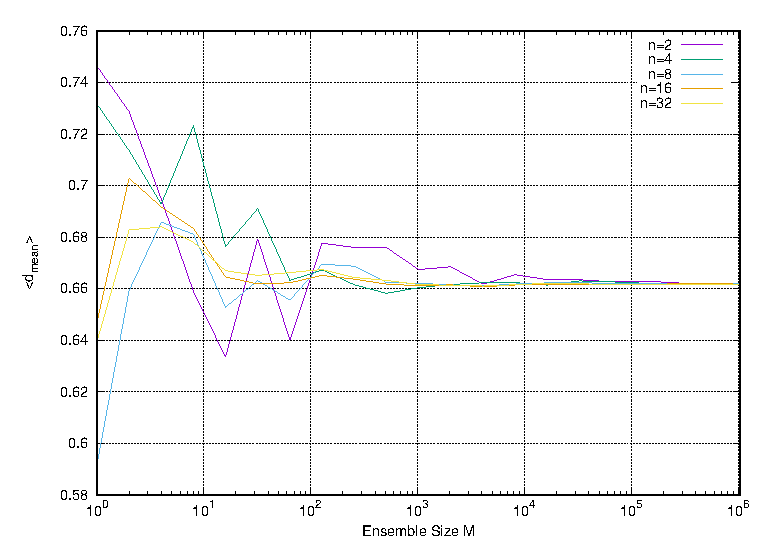
\includegraphics[scale=0.9]{figure1.eps} 
\end{center}
\caption{Convergence of $<d_{mean}>$ for different numbers of spheres $n$ and ensemble sizes $M$ (constant sphere radius $R=0.01$, constant box side length $L=1.0$).}
\label{fig:1}
\end{figure}


\section{Discussion}
As one would expect, it is evident that configurations with larger amounts of spheres $n$ converge quicker in the sense of ensemble size $M$ than configurations
with a low amount of spheres. This is because a higher $n$ "encourages" a uniform distribution of spheres in the box.
Also as expected, no matter what the number of spheres, all configurations eventually converge to the same value for $d_{mean}$ as the ensemble size $M$ increases.
Interestingly, the chosen approach of generating a complete configuration in a batch enforced rather low volume fractions $\nu$: Even when allowing for 
$10^6$ attempts to generate a valid configuration, values of $n \gtrapprox 60$ at a sphere radius of $R = 0.01$ often resulted in aborts for a lot (but not all)
initial seeds. Therefore, experiments were adjusted to keep $\nu \lessapprox 60 \cdot \frac{4}{3}\pi \frac{R^3}{L^3} \approx 2.5 \cdot 10^{-4}$.

\begin{thebibliography}{99}

\bibitem{herrmann}
	Herrmann, H. J.,
	Singer, H. M.,
	Mueller L.,
	Buchmann, M.-A.,\\
	\emph{Introduction to Computational Physics - Lecture Notes},\\
	ETH Zurich,\\
	2017.

\end{thebibliography}

\end{document}